When controlling the beam angle without any ball on the beam, we are using a simple PID controller.
When controlling the ball position along the beam, we are instead using a cascaded PID controller setup (see figure \ref{fig:cascaded_pid}).
Our implementation also allows for an additional beam angle reference to be supplied as a feed forward signal if desired, but in our final setup we do not make use of this.
\begin{figure}
\centering
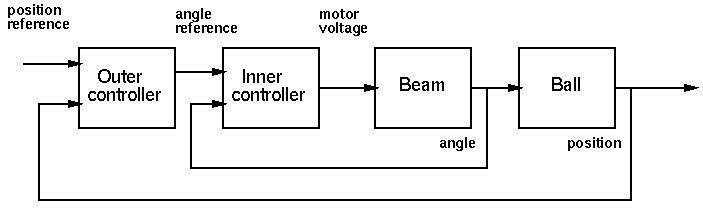
\includegraphics[width=\textwidth]{figures/block_diagram.png}
\caption{The cascaded PID setup.}\label{fig:cascaded_pid}
\end{figure}

As mentioned in the introduction, we have a sequence of tasks to be performed, and each of these (catching, weighing and delivering the ball) will be described in further detail in the following sections.

\subsection{Ball catching}\label{sec:ball_catching}
The ball magazine shown to the left of the beam in figure \ref{fig:process} is equipped with a ball dispatcher solenoid, which can be controlled from our program in order to push away a ball from the magazine.
For the ball to roll onto the beam however, the beam has to be aligned with the dispatcher.

Since the sensor measuring the beam angle is not very reliable, we make use of an additional optical sensor detecting when the beam is aligned with the dispatcher.
Starting at some underestimated angle near the dispatcher, the search for the correct beam angle is done by slowly increasing the beam angle until the optical sensor triggers. A small beam angle bias is then corrected for dispatching a ball.

\subsection{Ball weighing}\label{sec:ball_weighing}
When the ball rolls onto the beam (from the left), we want to determine its weight by measuring how much control signal\footnote{The control signal is essentially corresponding to a motor torque applied on the beam.} is necessary for keeping the ball near a certain weighing position.
We choose the weighing position to be to the right on the beam, and when controlling the ball to this position we are careful to avoid the ball rolling off the beam.
This is achieved by setting the ball position reference signal to a slowly increasing ramp, ending up at the weighing position.

The torque on the beam caused by a ball's gravity force $mg$ is\footnote{We are ignoring that the rotational center of the beam is not exactly at the mass centre of the ball when $x=0$, but actually slightly above.}
\[
\tau_{ball} = mgx
\]
where $x$ is the ball position. Letting $u$ denote the control signal, and assuming that $k_u u = \tau_{ball}$\footnote{The mass of the beam actually introduces an additional torque, since the beam is not rotating around its center of mass.
This can however be ignored for small beam angles, which is the case when balancing the ball at a certain position.} for some constant $k_u$, $mg/k_u$ can now be derived from $u$ and $x$.
Since $mg/k_u$ will always be the same for a particular ball, this measured quantity can now be used to indicate which ball is currently on the beam.

As the control signal $u$ can be very noisy, we apply lowpass filtering before deciding the ball size.
We are not as picky regarding the ball position however.
As $mg/k_u$ can be measured for any $x$, we do not need to wait for the controller to keep the ball entirely still at the weighing position before making the ball size decision.
This is implemented by having a high tolerance for the ball position, and reduces the running time of the weighing a lot.

\subsection{Ball delivery}\label{sec:ball_delivery}
Depending on the detected ball size, we now do different things according to the problem formulation in section \ref{sec:introduction}, explained in more detail in the following sections.

\subsubsection{Small ball}\label{sec:small_ball_delivery}
For the small ball to be rolled into the cup to the upper left from the beam, the ball is first stabilized at the weighing position in order to make the following actions more deterministic.
When stabilizing the ball, the tolerance is now much less as compared to when weighing.

After the ball is stabilized a heuristically pre-tuned angle reference trajectory (see figure \ref{fig:weighandthrowsmallball}) is applied, making the ball roll into the cup.
No ball position feedback is used.

\subsubsection{Medium ball}\label{sec:medium_ball_delivery}
If the ball is determined to have medium size, it is to be thrown to the right, away from the beam.
Before doing the throw however, the ball is moved to a "throw position" at the left end of the beam.
As for the weighing position, this has to be done carefully (by a suitable choice of reference, see figure \ref{fig:movemediumball}), avoiding the ball to roll off the beam.

When the ball is considered stationary at the throwing position, a pre-tuned angle reference trajectory throws the ball in the same manner as for the small ball described above. See figure \ref{fig:throwmediumball} for the reference appearance.

\subsubsection{Large ball}\label{sec:large_ball_delivery}
If the ball size is determined to be the largest one, a constant beam angle reference is simply applied, making the beam tilt and dropping the ball on the floor.









